\documentclass[a4paper,10.9pt]{article}
\usepackage[utf8]{inputenc}
\usepackage[T1]{fontenc}
\usepackage{fancyhdr} % pour personnaliser les en-têtes
\usepackage{lastpage}
\usepackage[frenchb]{babel}
\usepackage{amsfonts,amssymb}
\usepackage{amsmath,amsthm}
\usepackage{paralist}
\usepackage{xspace}
\usepackage{xcolor}
\usepackage{variations}
\usepackage{xypic}
\usepackage{eurosym,multicol}
\usepackage{graphicx}
\usepackage[np]{numprint}
\usepackage{hyperref} 
\usepackage{listings} % pour écrire des codes avec coloration syntaxique  

\usepackage{tikz}
\usetikzlibrary{calc, arrows, plotmarks,decorations.pathreplacing}
\usepackage{colortbl}
\usepackage{multirow}
\usepackage[top=1.5cm,bottom=1.5cm,right=1.5cm,left=1.5cm]{geometry}

\newtheorem{defi}{Définition}
\newtheorem{thm}{Théorème}
\newtheorem{thm-def}{Théorème/Définition}
\newtheorem{rmq}{Remarque}
\newtheorem{prop}{Propriété}
\newtheorem{cor}{Corollaire}
\newtheorem{lem}{Lemme}
\newtheorem{ex}{Exemple}
\newtheorem{cex}{Contre-exemple}
\newtheorem{prop-def}{Propriété-définition}
\newtheorem{exer}{Exercice}
\newtheorem{nota}{Notation}
\newtheorem{ax}{Axiome}
\newtheorem{appl}{Application}
\newtheorem{csq}{Conséquence}
\theoremstyle{definition}
\newtheorem{exo}{Exercice}


\newcommand{\vtab}{\rule[-0.4em]{0pt}{1.2em}}
\newcommand{\V}{\overrightarrow}
\renewcommand{\thesection}{\Roman{section} }
\renewcommand{\thesubsection}{\arabic{subsection} }
\renewcommand{\thesubsubsection}{\alph{subsubsection} }
\newcommand{\C}{\mathbb{C}}
\newcommand{\R}{\mathbb{R}}
\newcommand{\Q}{\mathbb{Q}}
\newcommand{\Z}{\mathbb{Z}}
\newcommand{\N}{\mathbb{N}}


\definecolor{vert}{RGB}{11,160,78}
\definecolor{rouge}{RGB}{255,120,120}
% Set the beginning of a LaTeX document
\pagestyle{fancy}


\begin{document}
	
\lhead{Lycée Le Maurice Genevoix}\chead{}\rhead{Année~2021-2022}\lfoot{M. Botcazou}\cfoot{\thepage/3}\rfoot{\textbf{Tourner la page S.V.P.}}\renewcommand{\headrulewidth}{0.4pt}\renewcommand{\footrulewidth}{0.4pt}

\hfill\\[-0.7cm]
$$	\fbox{\text{\Large{ \sc Devoir Maison à rendre pour le 03 janvier  2022 }}}$$



\quad \\\textbf{\textit{Note aux lecteurs:}} \textit{ce devoir maison devra être rédigé sur une copie avec un stylo de couleur foncé. La présentation et la qualité de rédaction seront un facteur important d'appréciation des copies.}

\begin{exo}\textit{\textbf{Les vecteurs, des bons outils pour faire de la physique:}}\\[0.5mm]

\noindent - Avant de commencer cet exercice, je vous invite à réaliser l'expérience suivante:\\

\noindent \textit{"Prenez dans votre main un crayon ou une gomme, ou une règle, ou encore quelque chose qui ne soit pas fragile.Tendez votre bras devant vous et ouvrez la main pour laisser tomber cet objet. Faite cette expérience plusieurs fois en fixant le mouvement de votre objet."}\\[0.5mm]

\noindent - Évidemment l'objet tombe, mais pourquoi? Un physicien vous dirait:\\[2mm]
\noindent \textit{"Mais c'est très simple... c'est à cause de la loi universelle de gravitation... le crayon est attiré vers la terre avec une force dépendant de la masse de la terre et de celle du crayon, inversement proportionnel à la distance au carré entre le crayon et le centre de la terre, moyennant une petite constante gravitationnelle..."}\\[2mm]
\noindent\underline{En résumé}: Une force attire le "crayon" vers le sol. Lorsque nous le lâchons, le crayon est mis en mouvement à cause de cette force. Cette force qui attire le crayon vers le sol, s'appelle la force de gravité terrestre, appelée aussi force de pesanteur terrestre.

\begin{defi}\quad\\
	\par $\bullet$ \quad Une \textbf{ force} correspond en physique à une action mécanique d'un objet sur un autre. L'unité de mesure d'une force est le \textbf{Newton}, référence au célèbre physicien britannique Isaac Newton (1643-1727).\\
	\par $\bullet$ \quad Une force qui agit sur un objet admet une \textbf{direction}, une \textbf{intensité}, un \textbf{sens} et un \textbf{point d'application}.   
\end{defi}  
\begin{prop}
	L'action des forces sur un objet peut créer du mouvement, elle peut entrainer une variation sur la vitesse de cet objet.
\end{prop}
\subsection*{Comment utiliser les vecteurs pour représenter des forces dans une situation physique?}
\noindent Une pomme est tranquillement accrochée dans un pommier, nous la regardons elle est immobile. En un instant elle se met en mouvement, elle se décroche de la branche et chute vers le sol. 
\section*{Une pomme accrochée dans un arbre :}

\textbf{QUESTIONS:}\\
\begin{enumerate}
	\item Notre pomme pèse 120 grammes.\\
	 Un physicien nous dit :~~\textit{"Chaque gramme de la pomme est attiré vers la terre avec une force de ~0.01~ Newton "}\\
	 \begin{enumerate}
	 	\item Quelle est l'intensité de la force de gravité terrestre subie par la pomme? Nous noterons $\V{G}$ la force de gravité terrestre subie par la pomme.
	 	\item En vous aidant du schéma 1 donné en Annexe, donnez la direction et le sens de la force de gravité subie par la pomme.\\
	 \end{enumerate} 
	 
	\item \begin{enumerate}
		\item Avec l'échelle d'un carreau pour ~0.4~Newton, donner le nombre de carreaux nécessaire pour représenter la force de gravité subie par la pomme.
		\item Représenter sur le schéma 1 à l'aide d'un vecteur qui part du point C, la force de gravité subi par la pomme.
	\end{enumerate}
	\item Au premier regard la pomme était immobile, cela signifie que la somme des forces subie par la pomme était nulle. Au départ, la branche exerce une force contraire qui retient la pomme. Un physicien nous dit :~~\textit{"Chaque gramme de la pomme est retenue par la branche avec une force de ~0.01~ Newton"} \\
	\begin{enumerate}
		\item Quelle est l'intensité de la force de retenue de la branche sur la pomme? Nous noterons $\V{R}$ la force de retenue de la branche.
		\item En vous aidant du schéma 1 donné en Annexe, donnez la direction et le sens de la force de retenue de la branche sur la pomme.\\
	\end{enumerate}
	\item
	 \begin{enumerate}
		\item Avec l'échelle d'un carreau pour ~0.4~Newton, donner le nombre de carreaux nécessaire pour représenter la force de retenue de la branche sur la pomme.
		\item Représenter sur le schéma 1 à l'aide d'un vecteur qui part du point A, la force de retenue de la branche sur la pomme.\\
	\end{enumerate}
	\item Quelles comparaisons pouvez-vous faire entre le vecteur ~$\V{G}$~ et le vecteur ~$\V{R}$~? \\Que pouvez-vous dire de la somme des vecteurs ~~$\V{G} \ + \ \V{R}$~~?
\end{enumerate}
\lhead{Lycée Le Maurice Genevoix}\chead{}\rhead{Année~2021-2022}\lfoot{M. Botcazou}\cfoot{\thepage/3}\rfoot{\textbf{}}\renewcommand{\headrulewidth}{0.4pt}\renewcommand{\footrulewidth}{0.4pt}
\section*{Une pomme qui chute vers le sol :}
\noindent Les fortes chaleurs de l'été et le vent fragilisent la résistance des branches. La force de retenue de la branche sur la pomme diminue en intensité avec le temps. Lorsque la sommes des forces subie par la pomme n'est plus nulle, la pomme se met en mouvement et chute vers le sol.\\

\textbf{QUESTIONS:}\\
\begin{enumerate}
	\item[6.] Notre pomme pèse toujours 120 grammes.\\
	\begin{enumerate}
		\item Quelle est l'intensité de la force de gravité terrestre subi par la pomme? Nous noterons encore $\V{G}$ la force de gravité terrestre.
		\item Représenter sur le schéma 2 à l'aide d'un vecteur qui part du point C, la force de de gravité subi par la pomme. Vous utiliserez la même échelle qu'aux questions précédentes.\\
	\end{enumerate} 
	\item[7.] Juste avant que la pomme ne tombe, un physicien nous dit : ~~\textit{"Chaque gramme de la pomme est maintenant retenue par la branche avec une force de ~0.005~ Newton"}\\ 
	\begin{enumerate}
		\item Quelle est l'intensité de la force de retenue de la branche sur la pomme à cet instant? Nous noterons encore $\V{R}$ la force de retenue de la branche.
		\item Représenter sur le schéma 2 à l'aide d'un vecteur qui part du point A, la force de retenue de la branche sur la pomme. Vous utiliserez la même échelle qu'aux questions précédentes.\\
	\end{enumerate}
	\item[8.] Quelles comparaisons pouvez-vous faire entre le vecteur ~$\V{G}$~ et le vecteur ~$\V{R}$~? \\Que pouvez-vous dire de la somme des vecteurs ~~$\V{G} \ + \ \V{R}$~~?\\
	\item[9.] Expliquer avec vos mots le lien qui existe dans cette situation, entre la somme  des vecteurs forces et la variation de mouvement de la pomme.
	
	
\end{enumerate}

\newpage
\lhead{Lycée Le Maurice Genevoix}\chead{}\rhead{Année~2021-2022}\lfoot{M. Botcazou}\cfoot{\thepage/3}\rfoot{\textbf{FIN}}\renewcommand{\headrulewidth}{0.4pt}\renewcommand{\footrulewidth}{0.4pt}
\section*{ANNEXE:}
\subsection*{Annexe 1:}
\begin{figure*}[!h]
	\centering
	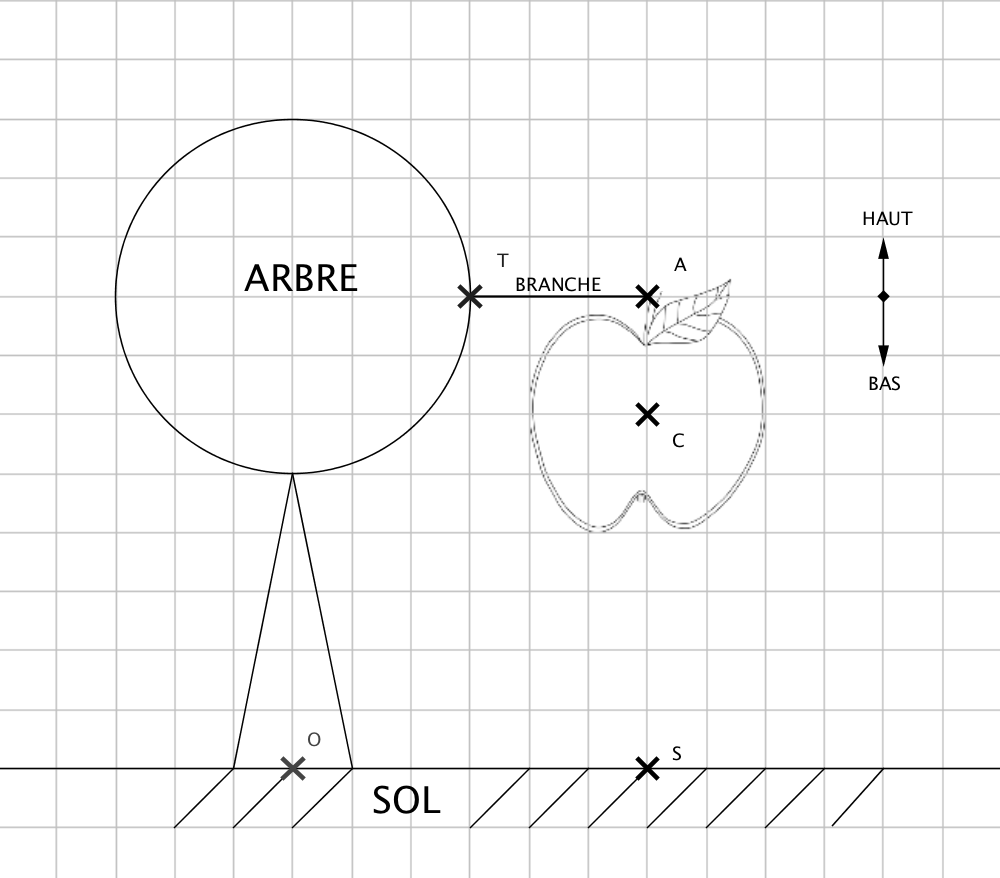
\includegraphics[scale=1.35]{DM_2.png}	
\end{figure*}
\subsection*{Annexe 2:}
  \begin{figure*}[!h]
    	\centering
    	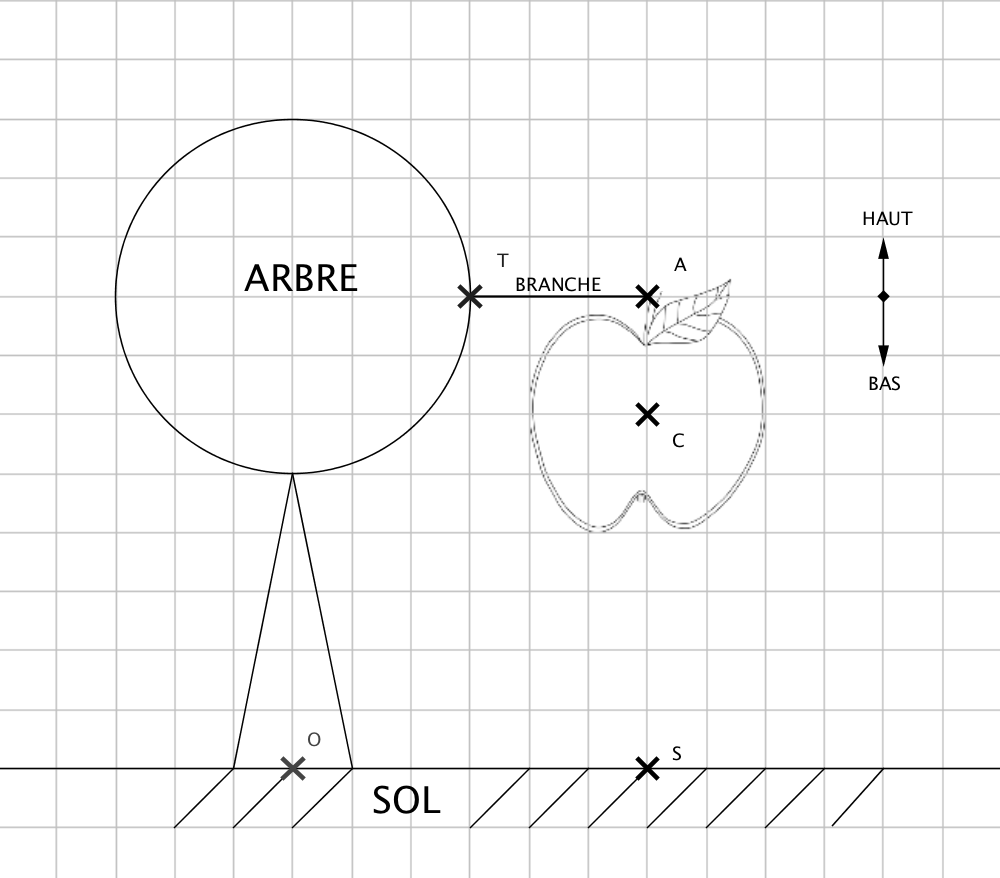
\includegraphics[scale=1.35]{DM_2.png}	
    \end{figure*}
\end{exo}
\end{document}